\documentclass[twoside,11pt]{article}
\usepackage[T1]{fontenc}
\usepackage{blindtext}
\usepackage{siunitx}
\sisetup{output-exponent-marker=\ensuremath{\mathrm{e}}}

% Any additional packages needed should be included after jmlr2e.
% Note that jmlr2e.sty includes epsfig, amssymb, natbib and graphicx,
% and defines many common macros, such as 'proof' and 'example'.
%
% It also sets the bibliographystyle to plainnat; for more information on
% natbib citation styles, see the natbib documentation, a copy of which
% is archived at http://www.jmlr.org/format/natbib.pdf

% Available options for package jmlr2e are:
%
%   - abbrvbib : use abbrvnat for the bibliography style
%   - nohyperref : do not load the hyperref package
%   - preprint : remove JMLR specific information from the template,
%         useful for example for posting to preprint servers.
%
% Example of using the package with custom options:
%
% \usepackage[abbrvbib, preprint]{jmlr2e}

\usepackage[preprint]{jmlr2e}

% Definitions of handy macros can go here

\newcommand{\dataset}{{\cal D}}
\newcommand{\fracpartial}[2]{\frac{\partial #1}{\partial  #2}}

% ================ START OF NON-TEMPLATE SETUP ================ %
\usepackage[dvipsnames]{xcolor}
\usepackage{amsmath,amssymb}
\usepackage{xfrac}

% Silence unneeded warnings.
\usepackage{silence}
\WarningFilter{caption}{Unknown document class}

% For drawing automata.
\usepackage{tikz}
\usetikzlibrary{arrows.meta,matrix,automata,shapes,positioning}
\tikzstyle{elbl} = [fill=white,inner sep=1pt,font=\footnotesize,>=stealth]

% For tables.
\usepackage{booktabs,multirow}
\usepackage{subcaption}
\usepackage[font=small,labelfont=bf]{caption}

% Useful shorthand.
\newcommand{\tsc}[1]{\textsc{#1}}
\newcommand{\ttt}[1]{\texttt{#1}}
\newcommand{\tbf}[1]{\textbf{#1}}

% Shorthand for MLRegTest factors.
\newcommand{\tttx}[1]{\ttt{#1}\xspace}
\newcommand{\Alpha}{\tttx{Alph}}
\newcommand{\Tier}{\tttx{Tier}}
\newcommand{\Class}{\tttx{Class}}
\newcommand{\kay}{\tttx{k}}
\newcommand{\jay}{\tttx{j}}
\newcommand{\eye}{\tttx{i}}
\newcommand{\TrainSize}{\tttx{TrainSize}}
\newcommand{\TestType}{\tttx{TestType}}
\newcommand{\NNType}{\tttx{NNType}}
\newcommand{\AlgoType}{\tttx{AlgoType}}

% Code repository url
\newcommand{\repo}{https://github.com/adil-soubki/mlrt}

% Use these to change spacing of lists.
\usepackage{enumitem}
\setlist[enumerate]{
    topsep=0pt,itemsep=-0.5ex,
    partopsep=0.5ex,parsep=0.5ex
}
\setlist[itemize]{
    topsep=0pt,itemsep=-0.5ex,
    partopsep=0.5ex,parsep=0.5ex,
    leftmargin=10pt
}

% Set the paper title here.
\newcommand{\papertitle}{Benchmarking State-Merging Algorithms for Learning Regular Languages}

% Notes.
\newcommand{\assign}[2]{\textcolor{#1}{(#2)}}
\newcommand{\note}[3]{{
    \normalfont
    \noindent
    \textcolor{#1}{\textbf{#2}: #3}
}}
\newcommand{\adil}[1]{\note{Orchid}{Adil}{#1}}
\newcommand{\jeff}[1]{\note{Green}{Jeff}{#1}}
% ================= END OF NON-TEMPLATE SETUP ================= %

% Heading arguments are {volume}{year}{pages}{date submitted}{date published}{paper id}{author-full-names}

\usepackage{lastpage}
\jmlrheading{23}{2022}{1-\pageref{LastPage}}{1/21; Revised 5/22}{9/22}{21-0000}{}

% Short headings should be running head and authors last names

\ShortHeadings{\papertitle}{}
\firstpageno{1}

\begin{document}

\title{\papertitle}

%\author{\name{~Anonymous~Review~Copy}}
\author{
    \name Adil Soubki
    \email asoubki@cs.stonybrook.edu\\
    \addr Department of Computer Science \\
    Institute for Advanced Computational Science \\
    Stony Brook University
    \AND
    \name Jeffrey Heinz
    \email jeffrey.heinz@stonybrook.edu\\
    \addr Department of Linguistics \\
    Institute for Advanced Computational Science \\
    Stony Brook University
}

\editor{}

\maketitle

% trailing '%' for backward compatibility of .sty file
\begin{abstract}%
  The state-merging algorithms RPNI, EDSM, and ALERGIA are tested on MLRegTest, a benchmark for the learning of regular languages \citep{heinz-etal-2022-mlregtest}. MLRegTest contains training, development, and test data for 1,800 regular languages, which themselves are from several well-studied subregular classes. The results show that there is large variation in the performance of these algorithms on the benchmark with EDSM performing the best overall. Furthermore, the mean accuracies on the test data for all three state-merging algorithms are less than the mean accuracies obtained by the neural networks \citet{heinz-etal-2022-mlregtest} studied. A further experiment augments the training data in MLRegtest with shorter strings and shows they dramatically improve the performance of the state-merging algorithms.
\end{abstract}

% \begin{keywords}
%   keyword one, keyword two, keyword three
% \end{keywords}

\section{Introduction}

This paper presents the results of three well-known state-merging algorithms on MLRegTest, a benchmark for the machine learning of sequential classifiers \citep{heinz-etal-2022-mlregtest}
% \footnote{The associated paper for this talk will be published on arXiv imminently for reviewers' reference.}.
MLRegTest contains training, development, and test sets from 1,800 regular languages organized into classes spanning several subregular regions.
The three algorithms tested are RPNI \citep{rpni-1992}, EDSM \citep{Lang1998}, and ALERGIA \citep{CarrascoOncina1994,carr99}. \citet{Higuera2010} provides a uniform presentation of these algorithms.\footnote{RPNI is an acronynm for ``Regular Positive and Negative Inference.''
EDSM is an acronym for ``Evidence Driven State Merging.'' Neither \citet{CarrascoOncina1994} (who named the algorithm) nor \citet{Higuera2010} explain whether ALERGIA is an acronym even though it is common in grammatical inference for `IA' to abbreviate ``Inference Algorithm.''}
The results of this investigation reveal that while there is large variation in the performance of these algorithms on the benchmark, EDSM overall performs the best.
However, the mean accuracies on the test data for all three state-merging algorithms are less than the mean accuracies obtained by the neural networks \citet{heinz-etal-2022-mlregtest} studied.

To some extent this is not too surprising given that the parameters of the neural networks numbered in the hundreds of thousands, and the state merging algorithms are much simpler. On the other hand, there are theoretical results for RPNI and ALERGIA (see \S\ref{sec:bg}) which would lead one to expect better performance.

We also observe that the shortest training strings in MLRegTest are of length 20. It may be that shorter strings are necessary for the state-merging algorithms to do well on the languages in MLRegTest. In the parlance of grammatical inference, characteristic samples for these languages may necessarily contain strings shorter than length 20. We therefore conducted additional experiments where the training sets in MLRegTest were augmented with fewer than 1,000 shorter strings and ran the state-merging algorithms again. The results are encouraging for EDSM and RPNI, which see a nearly 15 point improvement in accuracy. 
Obviously, it is important to also examine the impact of shorter strings on the performance of neural networks, a task left for future research.

All of the code used, data sets developed, and observations collected in this course of this research are freely available on \href{\repo}{GitHub}.\footnote{\href{\repo}{\repo}}.

\section{Learning Regular Languages with State Merging} \label{sec:bg}

This section provides an overview of RPNI, EDSM, and ALERGIA.
Readers are referred to \citet{Higuera2010} for details and \citet{Heinz-delaHiguera-vanZaanen-GICL} for additional discussion. RPNI, EDSM, and ALERGIA are state-merging algorithms. These algorithms and many other variants are implemented in the FlexFringe software package, which provides a customisable toolkit for state-merging \citep{flexfringe,flexfringe-short}.

RPNI and EDSM take as input a set of strings, each of which is labeled as to whether or not they belong to the target language, and outputs a finite state acceptor (FA) which classifies strings accordingly.
ALERGIA takes as input a similar set of labeled strings and outputs a probabilistic finite state acceptor (PFA) which assigns probabilities to strings.
To use ALERGIA for sequential classification when the training data contains both positive and negative examples, as we do here, the algorithm is applied to the positive strings to output a PFA for the positive strings $P$, and it is applied separately to the negative strings to output a PFA for the negative strings $N$.
These two machines together provide a classifier: given some string $x$, $P(x)$ is compared to $N(x)$ and $x$ is classified according to which is more likely.

% A prefix tree of these strings is constructed and the states in the tree are labeled as accepting or rejecting or left unlabeled.
A prefix tree of these input strings is constructed and the states are either left unmarked, or labeled as accepting or rejecting.
Subsequently, a search is conducted for pairs of states to merge.
RPNI, EDSM, and ALERGIA differ in both how this search is conducted and the decision procedure used to determine if a given pair of states should be merged.
We first illustrate the prefix tree, then explain state-merging, and finally discuss particulars of the search.

\begin{figure}
    \centering
    \begin{subfigure}[b]{0.32\textwidth}
        \centering
        \resizebox{\linewidth}{!}{
        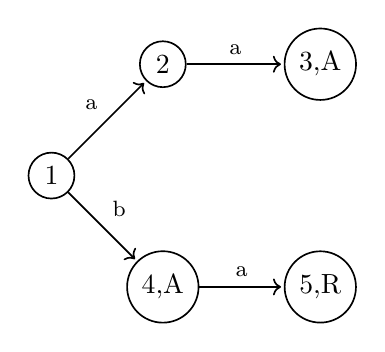
\begin{tikzpicture}
          [->,shorten >=1pt,node distance=20mm,semithick]
          \tikzstyle{every state}=[fill=white,draw=black,text=black,inner sep=3pt,minimum size=0pt]
        
          \node[state] (q1) {1};
          \node[state] (q2) [above right of = q1] {2};
          \node[state] (q3) [right of = q2] {3,A};
          \node[state] (q4) [below right of = q1] {4,A};
          \node[state] (q5) [right of = q4] {5,R};
        
          \path[->,auto,font=\footnotesize]
          (q1) edge[] node {a} (q2)
          (q1) edge[] node {b} (q4)
          (q2) edge[] node {a} (q3)
          (q4) edge[] node {a} (q5)
          ;
        \end{tikzpicture}
        }
        % \caption{The prefix tree built from positive strings are $\{aa,b\}$ and the negative strings are $\{ba\}$.}
        \caption{}
        \label{fig:pt}
    \end{subfigure}
    \begin{subfigure}[b]{0.32\textwidth}
        \centering
        \resizebox{\linewidth}{!}{
        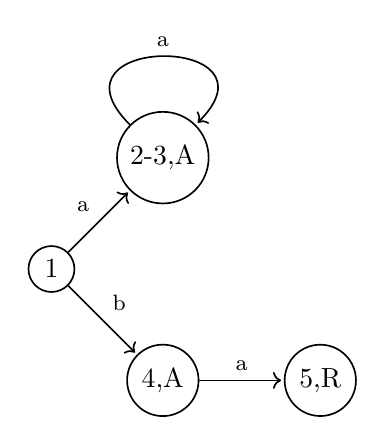
\begin{tikzpicture}
          [->,shorten >=1pt,node distance=20mm,semithick]
          \tikzstyle{every state}=[fill=white,draw=black,text=black,inner sep=3pt,minimum size=0pt]
        
          \node[state] (q1) {1};
          \node[state] (q2) [above right of = q1] {2-3,A};
        xw  \node[state] (q4) [below right of = q1] {4,A};
          \node[state] (q5) [right of = q4] {5,R};
        
          \path[->,auto,font=\footnotesize]
          (q1) edge[] node {a} (q2)
          (q1) edge[] node {b} (q4)
          (q2) edge[out=135,in=45,min distance=10mm,looseness=5] node {a} (q2)
          (q4) edge[] node {a} (q5)
          ;
        \end{tikzpicture}
        }  
        % \caption{The acceptor obtained by merging states 2 and 3 in the prefix tree.}
        \caption{}
        \label{fig:sm}
    \end{subfigure}
    \begin{subfigure}[b]{0.32\textwidth}
        \centering
        \resizebox{\linewidth}{!}{
        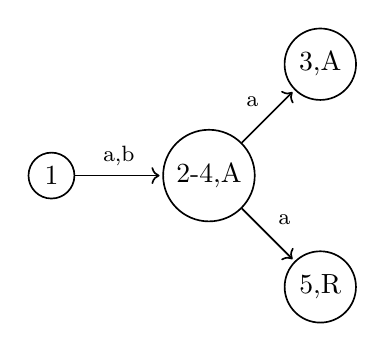
\begin{tikzpicture}
          [->,shorten >=1pt,node distance=20mm,semithick]
          \tikzstyle{every state}=[fill=white,draw=black,text=black,inner sep=3pt,minimum size=0pt]
        
          \node[state] (q1) {1};
          \node[state] (q2) [right of = q1] {2-4,A};
          \node[state] (q3) [above right of = q2] {3,A};
          \node[state] (q5) [below right of = q2] {5,R};
        
          \path[->,auto,font=\footnotesize]
          (q1) edge[] node {a,b} (q2)
          (q2) edge[] node {a} (q3)
          (q2) edge[] node {a} (q5)
          ;
        \end{tikzpicture}
        }
        % \caption{The acceptor obtained by merging states 2 and 4 in the prefix tree.}
        \caption{}
        \label{fig:nd}
    \end{subfigure}
    \caption{
        \tbf{(a)} The prefix tree built from positive strings are $\{aa,b\}$ and the negative strings are $\{ba\}$.
        \tbf{(b)} The acceptor obtained by merging states 2 and 3 in the prefix tree.
        \tbf{(c)} The acceptor obtained by merging states 2 and 4 in the prefix tree.
    }
\end{figure}

% \begin{figure}[ht]
%   \centering
% \begin{tikzpicture}
%   [->,shorten >=1pt,node distance=20mm,semithick]
%   \tikzstyle{every state}=[fill=white,draw=black,text=black,inner sep=3pt,minimum size=0pt]

%   \node[state] (q1) {1};
%   \node[state] (q2) [above right of = q1] {2};
%   \node[state] (q3) [right of = q2] {3,A};
%   \node[state] (q4) [below right of = q1] {4,A};
%   \node[state] (q5) [right of = q4] {5,R};

%   \path[->,auto,font=\footnotesize]
%   (q1) edge[] node {a} (q2)
%   (q1) edge[] node {b} (q4)
%   (q2) edge[] node {a} (q3)
%   (q4) edge[] node {a} (q5)
%   ;
% \end{tikzpicture}
%   \caption{The prefix tree built from positive strings are $\{aa,b\}$
%   and the negative strings are $\{ba\}$.}
%   \label{fig:pt}
% \end{figure}

% \begin{figure}[ht]
%   \centering
% \begin{tikzpicture}
%   [->,shorten >=1pt,node distance=20mm,semithick]
%   \tikzstyle{every state}=[fill=white,draw=black,text=black,inner sep=3pt,minimum size=0pt]

%   \node[state] (q1) {1};
%   \node[state] (q2) [above right of = q1] {2-3,A};
% xw  \node[state] (q4) [below right of = q1] {4,A};
%   \node[state] (q5) [right of = q4] {5,R};

%   \path[->,auto,font=\footnotesize]
%   (q1) edge[] node {a} (q2)
%   (q1) edge[] node {b} (q4)
%   (q2) edge[out=135,in=45,min distance=10mm,looseness=5] node {a} (q2)
%   (q4) edge[] node {a} (q5)
%   ;
% \end{tikzpicture}
%   \caption{The acceptor obtained by merging states 2 and 3 in the prefix tree.}
%   \label{fig:sm}
% \end{figure}

% \begin{figure}[ht]
%   \centering
% \begin{tikzpicture}
%   [->,shorten >=1pt,node distance=20mm,semithick]
%   \tikzstyle{every state}=[fill=white,draw=black,text=black,inner sep=3pt,minimum size=0pt]

%   \node[state] (q1) {1};
%   \node[state] (q2) [right of = q1] {2-4,A};
%   \node[state] (q3) [above right of = q2] {3,A};
%   \node[state] (q5) [below right of = q2] {5,R};

%   \path[->,auto,font=\footnotesize]
%   (q1) edge[] node {a,b} (q2)
%   (q2) edge[] node {a} (q3)
%   (q2) edge[] node {a} (q5)
%   ;
% \end{tikzpicture}
%   \caption{The acceptor obtained by merging states 2 and 4 in the prefix tree.}
%   \label{fig:nd}
% \end{figure}

Figure~\ref{fig:pt} presents an example prefix tree for a data sample where the positive strings are $\{aa,b\}$ and the negative strings are $\{ba\}$. In the figure, state 1 is the starting state and states are labeled A for accepting and R for rejecting.
To illustrate state-merging, consider Figure~\ref{fig:sm} where states 2 and 3 in the prefix tree above have been merged.
When two states are merged, the transitions must be preserved. The transition from state 2 to 3 in Figure~\ref{fig:pt} is now a self-loop in Figure~\ref{fig:sm}.
This is how generalization can occur.
Whereas the prefix tree recognizes only finitely many strings, the acceptor in Figure~\ref{fig:sm} recognizes infinitely many.
Furthermore, the merged state is accepting because it inherits that property from state 3.
Similarly, if state 2 was merged with state 5 the merged state would be rejecting because that property is inherited as well.
However, it is not possible to merge an accepting state with a rejecting state because those two properties are incompatible: a state cannot be both accepting and rejecting.

When two states are merged, non-determinism can occur.
Figure~\ref{fig:nd} shows the machine obtained by merging states 2 and 4 in the prefix tree, which introduces non-determinism.
RPNI, EDSM, and ALERGIA resolve non-determinism recursively by proceeding to merge states to eliminate any introduced non-determinism.
In this example, these algorithms would next attempt to merge states 3 and 5 to eliminate the non-determinism.
However, this attempt would fail because 3 is accepting and 5 is rejecting.
Consequently, the merging of states 2 and 4 would be rejected as well.

It is well known that for any regular language $L$, there exists a finite positive sample $S$ such that there is a way to merge states in the prefix tree $T$ of $S$ to yield an acceptor $A$ which recognizes $L$ exactly \citep[\S3.4.4]{Heinz-delaHiguera-vanZaanen-GICL}. The problem is knowing which states to merge. So how do RPNI, EDSM, and ALERGIA merge states?

RPNI, EDSM, and ALERGIA have procedures which tell them which states to try to merge.
If they can merge them they do, but if they cannot (because they lead to the merging of incompatible states) then they conclude that those two states must be distinct.
These procedures can be understood in terms of state coloring, a convention used to keep track of the state of search \citep{Higuera2010}.
A state is colored red if it will be included in the final automaton.
Initially, only the initial state of the prefix tree is colored red.
A state is colored blue if it is a candidate state to be merged with some red state.
Other states are colored white.
White states will eventually be colored blue, and then red.

The algorithms will attempt to merge each blue state $q$ with each red state.
If $q$ can merge with some red state, it is merged and that state stays red.
If $q$ cannot merge with any red state, then it becomes colored red and its successor states which are not red are colored blue.
State merging stops when all states are red.

RPNI conducts a breadth-first search of the prefix tree when trying to merge states. So given two potential merges -- blue state $b$ with red state $r$ or blue state $b'$ with red state $r'$ -- it will always choose the pair with blue state closest to the initial state.
If $b$ and $b'$ are equally close, it will choose the pair whose red state is closest to the initial state.
EDSM instead computes a score for all red and blue state pairs and first tries to merge the pair with the highest score.
The score of a merge is determined by the number of strings in the sample that would end in the merged state.
ALERGIA uses the Hoeffding statistical test to decide whether to merge states.  The states are merged if the Hoeffding test determines that the frequency distribution over the symbols on the outgoing transitions of the two states are not statistically significantly different.

To conclude this section, we summarize the theoretical and empirical results of these algorithms. RPNI provably identifies in the limit the class of regular languages from positive and negative data and runs in polynomial time and data \citep{rpni-1992}. Theoretical results are not known for EDSM but it outperformed other state merging algorithms in the Abbadingo One competition \citep{Lang1998}. ALERGIA provably identifies any deterministic PFA in the limit with probability one and runs in time polynomial in the size of the sample \citep{carr99,Higuera-Thollard-2000}.

\section{Experimental Setup}
This section provides a discussion of notable implementation details for the algorithms (\S\ref{sec:impl-details}), as well as an overview of the data set chosen for this study, MLRegTest (\S\ref{sec:mlregtest}), and concludes with a description of our experimental design and evaluation process (\S\ref{sec:evaluation}).

% We utilize the implementations of RPNI, EDSM, and ALERGIA provided by FlexFringe, a framework for implementing state-merging algorithms for automata learning \citep{flexfringe,flexfringe-short}. % These are trained on the small, medium, and large training data from MLRegTest \citep{heinz-etal-2022-mlregtest}.
% We benchmark these algorithms by training them on the small, medium, and large training data from MLRegTest and then evaluating the generated automata on the corresponding test data \citep{heinz-etal-2022-mlregtest}. This section provides a discussion of notable implementation details (\S\ref{sec:impl-details}), as well as an overview of MLRegTest (\S\ref{sec:mlregtest}), and a description of our evaluation process (\S\ref{sec:evaluation}).

\subsection{Implementation Details} \label{sec:impl-details}
The implementations of RPNI and ALERGIA provided by FlexFringe take minor departures from those described in the original papers. For RPNI, the original algorithm considers merging blue states in length-lexicographic order while FlexFringe instead uses a score when blue/red state pairs are equally distant from the initial state. Similarly, note that the version of ALERGIA we utilize is very similar to the original described by \citet{CarrascoOncina1994}, but with a few small changes as discussed by \citet[\S4.1]{flexfringe}.

% \begin{quote}
%     ``In FlexFringe, Alergia is implemented with the default score of summing up the differences between left-hand and right-hand sides of the above equation over all pairs of tested states. The larger these differences, the more similar are the distributions. In addition, this score prefers merges that merge many states during determinization.''
% \end{quote}

% Note that RPNI is actually this variant that sicco was talking about where is doesn't merge lexicographically. Note that ALERGIA is not the 1994 variant \citep{alergia-1994} but an updated version from the flexfringe paper \citep{flexfringe}.

\subsection{MLRegTest} \label{sec:mlregtest}
We train and test our models using MLRegTest \citep{heinz-etal-2022-mlregtest}, a benchmark data set for the learning of regular languages. It contains training, development, and test data with equally many positive and negative examples of strings from 1,800 regular languages across 16 different classes. The data is provided in small (1k), medium (10k), and large (100k) sizes with the smaller preparations fully contained in the each of the larger.

MLRegTest is designed to investigate a number of factors which may contribute to the learning performance. These factors are shown in Table \ref{tab:variables-table}, along with the values considered in this work. A regular language from the data set is uniquely identified by the factors alphabet size (\Alpha), tier size (\Tier), language class (\Class), factor width (\kay), threshold size (\jay), and index (\eye).

\begin{table}[!t]
    \centering
    \begin{tabular}{l p{10cm}}
        \toprule
        Factor Name & Description (Levels)                                                                                \\
        \midrule
        \Alpha      & Alphabet size (4, 16)                                                                               \\
        \Tier       & (3, 4, 7, 16)                                                                                       \\
        \Class      & Language class (SL, coSL, TSL, TcoSL, SP, coSP, LT, TLT, PT, LTT, TLTT, PLT, TPLT, SF, Zp, Reg)     \\
        \kay        & Factor width (0, 2, 3, 4, 5, 6)                                                                     \\
        \jay        & Threshold size (0, 1, 2, 3, 5)                                                                      \\
        \eye        & Index (0, 1, 2, 3, 4, 5, 6, 7, 8, 9)                                                                \\
        \TrainSize  & Size of training set (Small: 1k, Mid: 10k, Large: 100k)                                             \\
        \TestType   & Type of test set: whether strings are (S)hort or (L)ong, (R)andom or (A)dversarial (SR, SA, LR, LA) \\
        \AlgoType   & State merging algorithm (RPNI, EDSM, ALERGIA)                                                       \\
        \bottomrule
    \end{tabular}
    \caption{Factors comprising the experimental design.}
    \label{tab:variables-table}
\end{table}

The sixteen language classes in MLRegTest are organized according to descriptive complexity using logic and model-theoretic signatures of strings.
Five kinds of logic are considered: Monadic Second Order (MSO), First Order (FO), Propositional (Prop), Conjunctions of Negative literals (CNL) and Disjunctions of Positive Literals (DPL).
CNL and DPL are complements; both are fragments of Prop, which is properly contained in FO, which is a fragment of MSO.
Three basic model-theoretic signatures are considered: the successor model ($\triangleleft$), the tier-successor model ($\triangleleft_T$), and the precedence model ($<$), which at lower logical levels organize languages according to the concepts of substring, tier-substring, and subsequence, respectively.
A tier $T$ is a subset the alphabet $\Sigma$; they are the salient symbols. Non-tier elements are neutral and can be freely inserted or deleted \citep{Lambert2023}.

  \begin{table}[!t]
    \centering
    \begin{tabular}{cccc}
      \toprule
      Logic                 & Representation    & Language Name                     & Abbrevation          \\
      \midrule
      \multirow{3}{*}{MSO}  & $\triangleleft$   & \multirow{3}{*}{Regular}          & \multirow{3}{*}{Reg} \\
                            & $\triangleleft_T$ &           &                      \\
                            & $<$               &          &                      \\
      \midrule
      \multirow{3}{*}{FO}   & $\triangleleft$   & Locally Threshold Testable        & LTT                  \\
                            & $\triangleleft_T$ & Tier Locally Threshold Testable   & TLTT                 \\
                            & $<$               & Star-Free                         & SF                   \\
      \midrule
      \multirow{3}{*}{Prop} & $\triangleleft$   & Locally Testable                  & LT                   \\
                            & $\triangleleft_T$ & Tier Locally Testable             & TLT                  \\
                            & $<$               & Piecewise Testable                & PT                   \\
      \midrule
      \multirow{3}{*}{CNL}  & $\triangleleft$   & Strictly Local                    & SL                   \\
                            & $\triangleleft_T$ & Tier Strictly Local               & TSL                  \\
                            & $<$               & Strictly Piecewise                & SP                   \\
      \midrule
      \multirow{3}{*}{DPL}  & $\triangleleft$   & Complement of Strictly Local      & coSL                 \\
                            & $\triangleleft_T$ & Complement of Tier Strictly Local & coTSL                \\
                            & $<$               & Complement of Strictly Piecewise  & coSP                 \\
      \bottomrule
    \end{tabular}
    \caption{Logical characterizations and names of classes in MLRegTest.}
    \label{tab:classes}
  \end{table}

Choice of logic and model-theoretic signature define a logical language, whose formulas define formal languages.
At the highest level, MSO, these converge to the regular languages (Reg): MSO($\triangleleft$) = MSO($\triangleleft_T$) for all $T$ = MSO($<$).
MLRegTest considers an additional subclass of purely periodic languages they call Zp.\footnote{Examples include languages like $\{ w : |w|_a \mod 2 = 0\}$, i.e. the language whose words contain an even number of $a$ symbols.}
  At the FO level, the classes of languages defined by the logical languages are nested: FO($\triangleleft$) $\subsetneq$ FO($\triangleleft_T$) for all $T$ $\subsetneq$ FO($<$).
  At the propositional level we have Prop($\triangleleft$) is properly included by Prop($\triangleleft_T$), but both are incomparable with Prop($<$).
  An analgous relationship holds for CNL and DPL: if X$\in$\{CNL, DPL\}, it holds that X($\triangleleft$) is properly included by X($\triangleleft_T$), but both are incomparable with. X($<$).
  Many of these classes are well-studied and go by the names shown in Table~\ref{tab:classes}. Overviews of these classes and their relationships are discussed by \citet{McNaughtonPapert1971, Thomas1982, Thomas1997, RogersPullum2011, Rogers-HeinzEtAl-2013-CSC, rogers-lambert-2019-classes}. \citet{Lambert+2021-TESRL} discusses aspects of many of these classes learnability.

  Some of these are are known by other names. For example, what is called coSP here is also known as the $\sfrac{1}{2}$ level of the Straubing Hierarchy \citep{Straubing1985,PinWeil1997}.
  To this list of thirteen classes, MLRegTest also includes Piecewise Locally Testable (PLT) langauges given by Prop($<,\triangleleft$) and Tier Piecewise Locally Testable (TPLT) langauges given by Prop($<,\triangleleft_T$).
  While both of these classes are contained within FO($<$), it is the case that Prop($<,\triangleleft$) properly contains ($\triangleleft$), and Prop($<,\triangleleft_T$) properly contains ($\triangleleft_T$).
  \citet{heinz-etal-2022-mlregtest} verify that the languages representing a class A in MLRegTest belong to A and do not belong to any class B, where B is a subclass of A or is incomparable with A.
  We refer the reader to \citet{heinz-etal-2022-mlregtest} for additional details regarding these parameters.

MLRegTest contains four variations of testing data based on the length of the strings generated from the language (short or long) and the method of generation (random or adversarial). The short testing data contains equally many strings of all lengths between 20 and 29 whereas the long shifts this to be between 31 and 50. Similarly, the random test sets were sampled randomly without replacement while the adversarial test sets pair each positive example with a corresponding negative example such that the edit distance is one.

Our experiments are not conducted on the entirety of MLRegTest. In particular, we excluded languages with an alphabet of size 64. This is because it was discovered that the data sets of those languages were confounded by an error likely introduced by unicode normalization. Therefore the total number of languages in our study is 1,140 with every class represented.

\subsection{Evaluation} \label{sec:evaluation}
% We report the accuracy of the three models across several dimensions \adil{which ones? write here.} of the MLRegTest data set.

% To analyze the results, we follow the methods used by \citet{heinz-etal-2022-mlregtest}.

As advocated by \citet{Demsar2006} and \citet{Stapor2017} and employed by \citet{heinz-etal-2022-mlregtest}, we utilize non-parametric methods in our analysis. 
This minimizes the assumptions made about our data, as no distribution is required, while still allowing us to assign rankings to the variables under question. We report aggregate accuracy for the models as the primary measurement of performance. 
A model in our experiments is specified by the choice of regular language, size of the training data, and algorithm for building the automata. 
As a result, we aimed to generate 1,140 (regular languages) $\times$ 3 (training data sizes) = 3,420 models for each algorithm, each of which would be evaluated on 4 test sets, yielding 13,680 observations per algorithm.
We achieved this goal with EDSM and RPNI, but only obtained 11,136 observations for ALERGIA because it was time-intensive.

These observations are then aggregated over the variables \Tier, \kay, \jay, \eye and \Alpha. The analysis presented in \S\ref{sec:results} holds these as blocking variables, while considering factors such as \Class, \TrainSize, \TestType, and \AlgoType as treatment variables for which to compute average accuracy over. The Friedman rank sum test is used to determine if the factor being held for treatment contributes significantly to predicting model accuracy by holding the null hypothesis that all variations of the value contribute equally. We conduct additional analysis using the Nemenyi-Wilcoxon-Wilcox all-pairs test to identify exactly which pairs differ significantly.

Because EDSM, RPNI, and ALERGIA return finite state machines, these can be compared with the minimal deterministic finite state acceptors for the languages in MLRegTest. 
There are many forms this comparison can take. We chose to compare the sizes of the finite state machines as a first step. 
In future work, this analysis can be refined, examining other details such as the subset relationships of the corresponding languages.

% REWRITE: Our experimental design and statistical analysis follows the approaches advocated by \citet{Demsar2006} and \citet{Stapor2017}. We form a full factorial design by aggregating the variables \Tier{}, \kay{}, \jay{}, and \eye{}. Specifically, each cell in the design is specified by the factors \Alpha{}, \Class{}, \TrainSize{}, \TestType{}, and \NNType{}, and is an average of accuracy scores from observations that have different values of \Tier{}, \kay{}, \jay{}, and \eye{}. The full factorial design thus has 2,880 aggregated observations and makes possible repeated-measures non-parametric statistical tests, in particular the Friedman test \citep{Demsar2006,Stapor2017}. Indeed, any of the five factors \Alpha{}, \Class{}, \TrainSize{}, \TestType{}, or \NNType{} can be considered a \textit{treatment} variable while the remaining four form \textit{blocking} variables. We use the Friedman test to ask whether any of the treatment levels differ as predictors of model accuracy (\S\ref{sec:res}). In those cases that we reject the Friedman test null hypothesis of equal treatment effects, we conduct post hoc analyses using the Nemenyi-Wilcoxon-Wilcox all-pairs test to determine precisely where the significant differences exist \citep{Pereira+2015,Singh+2016}.




% With the exception of Cohen's $d$, which is used to quantify effect size, non-parametric methods are preferred in our analysis. This minimizes the assumptions made about our data, as no distribution is assumed, while still allowing us to assign rankings to the a

% Why non-parametric tests? Why just report accuracy? Etc...

% \subsubsection{Nemenyi-Wilcoxon-Wilcox All-Pairs Test}
% \subsubsection{Friedman Rank Sum Test}

\section{Results} \label{sec:results}
% [ ] Correlation between Small and Mid results.
%   [ ] If correlated we can just leave out the large.
% [ ] Correlation of Medium to Large with the ALERGIA that we have.
% [ ] 3x3 table (Small/Mid/Large) vs (RNPI/EDSM/ALERGIA) [See table 23]
% [ ] Reference the MLRegTest paper for tables to include.
% We follow a similar analysis to \citet{heinz-etal-2022-mlregtest} so our results on state-merging algorithms can be directly compared the performance of neural networks presented there.
We follow a similar analysis to \citet{heinz-etal-2022-mlregtest} so that their results on neural networks can be directly compared to the performance of the state-merging algorithms presented here.

\subsection{Training Size}
As the training data is nested such that increasing the size strictly increases the data seen, we expect the models trained on the larger splits to improve in accuracy.

% 20230311
% Large 0.662332402874217
% Mid   0.634866450954861
% Small 0.592576732783565
% Friedman chi-squared = 675.21, df = 2, p-value < 2.2e-16
\begin{table}[ht]
  \centering
  \begin{tabular}{lll}
    \toprule
    \textbf{Small} & \textbf{Mid} & \textbf{Large} \\
    0.585          & 0.624        & 0.655          \\
    \bottomrule
  \end{tabular}
  \caption{Average accuracy by \ttt{TrainSize}.}
  \label{tab:train-size}
\end{table}

As can be seen in Table \ref{tab:train-size}, the accuracy of the models does indeed increase on average with the size of the training data. 
The Friedman rank sum test also finds that varying the size of the training data leads to statistically significant differences in model performance (Friedman chi-squared = 542.58, df = 2, p-value $<$ \num{2.2e-16}). 
The Nemenyi-Wilcoxon-Wilcox test similarly rejects the null hypothesis with p-value at or below $<$ \num{2.9e-14} for all pairs. 
This is a good sanity check to ensure the integrity of the experimental setup and analysis pipeline.

Nonetheless, it was surprising that even on the Large training set the mean accuracy was not particularly high.
It is puzzling that these algorithms do not perform as well we might expect, even when trained on the large test sets. 
After all, it has been proven that RPNI will identify the target language in the limit provided the input data includes a characteristic sample. 
EDSM uses heuristics to guide its search, so no theoretical results exits, but analysis of ALERGIA does provide similar learnability results (see also \citet{Higuera-Thollard-2000,clarkthollard04}). 
The answer must be the large data sets do not include a characteristic sample. 
One reason may be that the shortest strings in the training sets in MLRegTest are at least of length 20. If the characteristic samples for the regular languages in MLRegTest necessarily contains strings of shorter lengths, then these algorithms will not achieve exact identification. 
Therefore, follow-up experiments which included shorter strings are reported in Section~\ref{sec:shorttrain}. 
The results of these experiments are encouraging.

\subsection{Test Set Type}
We turn our attention to the effect of \TestType on model accuracy. Table \ref{tab:test-type-avg} shows the average accuracy scores for each preparation of test data.

% 20230311
% LA 0.546698688527603
% LR 0.701951986591829
% SA 0.552585702248579
% SR 0.71846440478218
% Friedman chi-squared = 1131.7, df = 3, p-value < 2.2e-16
\begin{table}[ht]
  \centering
  \begin{tabular}{llll}
    \toprule
    \textbf{LA} & \textbf{SA} & \textbf{LR} & \textbf{SR} \\
    0.534       & 0.539       & 0.696       & 0.718       \\
    \bottomrule
  \end{tabular}
  \caption{Average accuracy by \ttt{TestType}.}
  \label{tab:test-type-avg}
\end{table}

Visually, the differences in scores look significant and the Friedman rank sum test confirms this suspicion by rejecting the null hypothesis that performance across test types is the same (Friedman chi-squared = 782.96, df = 3, p-value $<$ 2.2e-16). 
Additional analysis using the Nemenyi-Wilcoxon-Wilcox all-pairs test finds that all four preparations of test data differ significantly from each other at or below 1.9e-09.
% A summary is presented in Figure \ref{fig:test-type}.
These findings are consistent with the results on neural network architectures presented by \citet{heinz-etal-2022-mlregtest}.

% 20230311
%    LA      LR      SA
% LR < 2e-16 -       -
% SA 5.3e-14 < 2e-16 -
% SR < 2e-16 1.8e-12 < 2e-16
% \begin{table}[ht]
%     \centering
%     \begin{tabular}{llll}
%     \hline
%                 & \textbf{LA}  & \textbf{LR} & \textbf{SA} \\
%     \hline
%     \textbf{LR} & $< 2e-16$      & $-$           & $-$ \\
%     \textbf{SA} & $5.3e-14$      & $< 2e-16$     & $-$ \\
%     \textbf{SR} & $< 2e-16$      & $1.8e-12$     & $< 2e-16$ \\
%     \hline
%     \end{tabular}
%     \caption{Nemenyi-Wilcoxon-Wilcox all-pairs test results comparing \ttt{TestType}.}
%     \label{tab:test-type-nww}
% \end{table}

% Not doing Cohen's d test.
% \begin{table}[ht]
%     \centering
%     \begin{tabular}{clc}
%         \hline
%         \textbf{Pair} & \textbf{Effect Size} & \textbf{Interpretation} \\
%         \hline
%         SR, LR & $0.105 \pm 0.025$ & Negligible \\
%         LR, SA & $1.169 \pm 0.027$ & Large  \\
%         SA, LA & $0.060 \pm 0.025$ & Negligible \\
%         \hline
%     \end{tabular}
%     \caption{Cohen's $d$ test comparing \ttt{TestType}.}
%     \label{tab:test-type-cohen}
% \end{table}

% \begin{figure}[ht]
%     \centering
%     \includegraphics[width=\textwidth]{images/accuracy-by-class-and-training-set-size.jpeg}
%     \caption{Accuracy by \ttt{Class} and \ttt{TestType}. \adil{UPDATE THIS.}}
%     \label{fig:test-type}
% \end{figure}

\begin{figure}[ht]
    \centering
    \includegraphics[width=\textwidth]{images/accuracy-by-class-and-test-type-og.jpg}
    \caption{Accuracy by \Class and \TestType.}
    \label{fig:test-type}
\end{figure}

\subsection{Language Class}
In this section we investigate the impact that \Class has on model accuracy. To do this, we consider two groupings of the 16 language classes based on the weakest logic capable of describing the language (CNL, DPL, PROP, FO, REG) and the order relation used to represent strings from that language (successor, precedence, tier-successor).

\subsubsection{Logical Level}

% cnl = c("SL", "SP", "TSL")
% dpl = c("coSL", "coSP", "TcoSL")
% prop = c("LT", "LP", "PT", "TLT", "TLP")
% fo = c("LTT", "TLTT", "SF")
% reg = c("Zp", "Reg")
\begin{table}[t]
    \centering
    \begin{tabular}{lll}
    \toprule
    \tbf{Abbrev.} & \tbf{Logical Level} & \tbf{Lang. Classes} \\
    \midrule
    CNL & Conjunction of Negative Literals & SL, SP, TSL \\
    DPL & Disjunction of Positive Literals & coSL, coSP, TcoSL \\
    PROP & Propositional & LT, PLT, PT, TLT, TPLT \\
    FO & First Order & LTT, TLTT, SF \\
    REG & Monadic First Order & Zp, Reg \\
    \bottomrule
    \end{tabular}
    \caption{Language classes grouped by logical level.}
    \label{tab:logical-level}
\end{table}

The language classes grouped by their logical level are shown in Table \ref{tab:logical-level}. If we find a significant difference in accuracy based on the logical level, one might expect accuracy to decrease as we ascend to more expressive logical levels.

% \begin{table}[htb]
% \begin{minipage}[t]{.5\linewidth}
%     \centering
%     \begin{tabular}[t]{lllll}
%     \toprule
%     \tbf{REG} & \tbf{PROP} & \tbf{DPL} & \tbf{CNL} & \tbf{FO} \\
%     0.595     & 0.620      & 0.628     & 0.630     & 0.649    \\
%     \bottomrule
%     \end{tabular}
%     \caption{Average accuracy by logical level.}
%     \label{tab:logical-level-avg}
% \end{minipage}%
% \begin{minipage}[t]{.5\linewidth}
%     \centering
%     \begin{tabular}[t]{cllll}
%     \toprule
%                & \tbf{CNL} & \tbf{DPL} & \tbf{FO} & \tbf{PROP} \\
%     \midrule
%     \tbf{DPL}  & 0.510     & $-$       & $-$      & $-$        \\
%     \tbf{FO}   & 0.774     & 0.048     & $-$      & $-$        \\
%     \tbf{PROP} & 0.084     & 0.878     & 0.002    & $-$        \\
%     \tbf{REG}  & 0.016     & 0.544     & $1.9e-4$ & 0.978      \\
%     \bottomrule
%     \end{tabular}
%     \caption{Nemenyi-Wilcoxon-Wilcox all-pairs test results comparing by logical level.}
%     \label{tab:logical-level-nww}
% \end{minipage} 
% \caption{Global caption}
% \end{table}

% [20230311] - Logical Level (Average)
% CNL  0.642004600352478
% DPL  0.636213478091551
% FO   0.652654323343414
% PROP 0.633079813829647
% REG  0.596788202279202
% Friedman chi-squared = 73.509, df = 4, p-value = 4.117e-15
\begin{table}[ht]
  \centering
  \begin{tabular}{lllll}
    \toprule
    \tbf{REG} & \tbf{PROP} & \tbf{DPL} & \tbf{CNL} & \tbf{FO} \\
    0.595     & 0.620      & 0.628     & 0.630     & 0.649    \\
    \bottomrule
  \end{tabular}
  \caption{Average accuracy by logical level.}
  \label{tab:logical-level-avg}
\end{table}

The Friedman test finds that logical level is a significant factor in predicting accuracy (Friedman chi-squared = 25.133, df = 4, p-value = 4.73e-05).
%While we do find visually that ascending the hierarchy of logical levels (CNL $\sim$ DPL $<$ PROP $<$ FO $<$ REG) does tend to reduce accuracy, the relationship is not exactly clear.

% [20230311] - Logical Level (NWW)
%      CNL     DPL     FO      PROP
% DPL  0.00236 -       -       -
% FO   0.98576 0.00029 -       -
% PROP 0.00121 0.99980 0.00013 -
% REG  1.1e-10 0.01452 2.6e-12 0.02488
\begin{table}[ht]
    \centering
    \begin{tabular}{cllll}
    \toprule
               & \tbf{CNL} & \tbf{DPL} & \tbf{FO} & \tbf{PROP} \\
    \midrule
    \tbf{DPL}  & 0.510     & $-$       & $-$      & $-$        \\
    \tbf{FO}   & 0.774     & 0.048     & $-$      & $-$        \\
    \tbf{PROP} & 0.084     & 0.878     & 0.002    & $-$        \\
    \tbf{REG}  & 0.016     & 0.544     & $1.9e-4$ & 0.978      \\
    \bottomrule
    \end{tabular}
    \caption{Nemenyi-Wilcoxon-Wilcox all-pairs test results comparing by logical level.}
    \label{tab:logical-level-nww}
\end{table}
Interrogating the Nemenyi-Wilcoxon-Wilcox all-pairs test tells a different story from predictions based on logical complexity. While REG is generally the hardest to learn, there are few significant differences anywhere. The only ones which appear significant are properly FO languages from properly propositional ones and properly regular ones. This differs from the analysis by \citet{heinz-etal-2022-mlregtest} on neural network architectures which found everything FO and below to be indistinguishable.
% \adil{this is a weird result... maybe I should check the analysis without alergia and see if it persists?}

\subsubsection{Order Relation}

Next we consider the language classes grouped by order relation as shown by Table \ref{tab:order-relation}. From the results above we might expect OTHER to obtain the lowest accuracy, as it contains the regular class, followed by the rest.

% succ = c("SL", "coSL", "LT", "LTT")
% prec = c("coSP", "PT", "SF", "SP")
% tsucc = c("TcoSL", "TLT", "TLTT", "TSL")
\begin{table}[ht]
  \centering
  \begin{tabular}{lll}
    \toprule
    \tbf{Abbrev.} & \tbf{Order Relation} & \tbf{Lang. Classes}   \\
    \midrule
    SUCC          & Successor            & SL, coSL, LT, LTT     \\
    PREC          & Precedence           & coSP, PT, SF, SP      \\
    TSUCC         & Tier Successor       & TcoSL, TLT, TLTT, TSL \\
    OTHER         & Other                & LP, TLP, Reg, Zp      \\
    \bottomrule
    \end{tabular}
    \caption{Langauge classes grouped by order relation.}
    \label{tab:order-relation}
\end{table}

Consulting the Friedman rank sum test finds order relation to be a significant factor (Friedman chi-squared = 13.95, df = 3, p-value = 0.002974). Further examining the p-values from the Nemenyi-Wilcoxon-Wilcox all-pairs test, see Table \ref{tab:successor-nww}, finds significant differences between successor and tier-successor languages.
%Additionally, PREC and OTHER are not differentiable by this measure but the remaining pairs have low p-values which may be considered significant.

% \begin{table}[!htb]
% \begin{subtable}[t]{.5\linewidth}
%     \centering
%     \begin{tabular}[t]{llll}
%     \toprule
%     \tbf{OTHER} & \tbf{SUCC} & \tbf{PREC} & \tbf{TSUCC} \\
%     \midrule
%     0.616       & 0.622      & 0.633      & 0.635       \\
%     \bottomrule
%     \end{tabular}
%     \caption{}
%     \label{tab:successor-avg}
% \end{subtable}%
% \begin{subtable}[t]{.5\linewidth}
%     \centering
%     \begin{tabular}[t]{clll}
%     \toprule
%                 & \tbf{OTHER} & \tbf{PREC} & \tbf{SUCC} \\
%     \midrule
%     \tbf{PREC}  & 0.569       & $-$        & $-$        \\
%     \tbf{SUCC}  & 0.041       & 0.527      & $-$        \\
%     \tbf{TSUCC} & 0.836       & 0.144      & 0.003      \\
%     \bottomrule
%     \end{tabular}
%     \caption{}
%     \label{tab:successor-nww}
% \end{subtable}
% \caption{\tbf{(a)} Average accuracy by successor relation. \tbf{(b)} Nemenyi-Wilcoxon-Wilcox all-pairs test results comparing by successor relation.}
% \end{table}

% [20230311] - Successor Relation (Average)
% OTHER 0.626926266715267
% PREC  0.646035515923177
% SUCC  0.624930448930227
% TSUCC 0.647104313954457
% Friedman chi-squared = 34.297, df = 3, p-value = 1.715e-07
\begin{table}[ht]
  \centering
  \begin{tabular}{llll}
    \toprule
    \tbf{OTHER} & \tbf{SUCC} & \tbf{PREC} & \tbf{TSUCC} \\
    0.616       & 0.622      & 0.633      & 0.635       \\
    \bottomrule
  \end{tabular}
  \caption{Average accuracy by successor relation.}
  \label{tab:successor-avg}
\end{table}

% [20230311] - Successor Relation (NWW)
%       OTHER PREC  SUCC
% PREC  1.000 -     -
% SUCC  0.023 0.020 -
% TSUCC 0.014 0.017 2.9e-08
\begin{table}[ht]
    \centering
    \begin{tabular}{clll}
    \toprule
                & \tbf{OTHER} & \tbf{PREC} & \tbf{SUCC} \\
    \midrule
    \tbf{PREC}  & 0.569       & $-$        & $-$        \\
    \tbf{SUCC}  & 0.041       & 0.527      & $-$        \\
    \tbf{TSUCC} & 0.836       & 0.144      & 0.003      \\
    \bottomrule
    \end{tabular}
    \caption{Nemenyi-Wilcoxon-Wilcox all-pairs test results comparing by successor relation.}
    \label{tab:successor-nww}
\end{table}

% \subsection{Alphabet Size}

% [20230311]
% 4  0.633698476512685
% 16 0.609613977913287
% 64 0.646463132186671
% \begin{table}[ht]
%     \centering
%     \begin{tabular}{c|lll}
%     \hline
%     \textbf{Alphabet Size} & 4 & 16 & 64 \\
%     \textbf{Mean Accuracy} & 0.634 & 0.610 & 0.646 \\
%     \hline
%     \end{tabular}
%     \caption{Average accuracy by \Alpha.}
%     \label{tab:alphabet-size-avg}
% \end{table}

\subsection{Analysis by Machine Sizes}

We now turn away from the parametric statistical tests to qualitatively inspect the sizes of the learned machines relative to the source machines used for generating the data sets. 
When state-merging algorithms return a machine $M$ with more states than the target machine, it means not enough states were merged, and therefore $M$ makes more distinctions than necessary (a kind of overfitting). 
On the other hand, if $M$ is smaller than the target, it means too few distinctions were made and $M$ overgeneralizes. 
On average the learned FAs are larger than the data source FAs in roughly $\sfrac{3}{4}$ experiments, smaller in about $\sfrac{1}{4}$, and exactly the same size in the remaining 2.5\% of cases. The appendix includes figures which give more details on this analysis.

% \begin{table}[!htb]
% \centering
% \begin{tabular}{lrrr}
% \toprule
%       & \tbf{ALERGIA} & \tbf{EDSM} & \tbf{RPNI} \\
% \midrule
% \tbf{Small} & 0.96 & 5.02   & 8.17 \\
% \tbf{Mid}   & 3.07 & 25.02  & 39.41 \\
% \tbf{Large} & 9.00 & 149.10 & 227.38 \\
% \bottomrule
% \end{tabular}
% \caption{Learned machine size by training data.}
% \label{tab:size-by-train}
% \end{table}

For EDSM and RPNI the learned machines are much larger, averaging state counts that are 59.71 (std=163.18, median=6.63) and 91.66 (std=213.32, median=13.15) times larger, respectively. While ALERGIA also learns machines that are larger than the source, they average a relatively modest 3.28 (std=6.32, median=1.00) times increase in size.
As expected, larger training data sets resulted in models with larger numbers of states  (see Figure~\ref{fig:size-by-data} in the appendix).
These size increases were especially notable in the Zp languages where EDSM and RPNI averaged size factors of 231.11 and 311.44 each. Meanwhile, machines trained on SP and coSP languages had mean factors (ALERGIA=1.38, EDSM=18.20, RPNI=33.04) which were among the lowest. This wide range in variability results in the large standard deviations seen.

% Finally, we compared accuracy to the size of the target machine.
We also investigated the relationship between learned machine size and accuracy. This revealed that, across all test types, larger machines were less accurate for EDSM and RPNI. However, this trend was reversed for ALERGIA which saw larger machines perform better (see Figure~\ref{fig:acc-by-size} in the appendix). 
When the machine sizes exactly matched the source, the accuracy was higher, but not perfect. In these cases the average accuracies were 0.89 (std=0.19, median=1.00) for EDSM, 0.94 (std=0.15, median=1.00) for RPNI, and 0.56 (std=0.10, median=0.50) for ALERGIA. It is curious that ALERGIA sees essentially no improvement in this case. In fact, despite the median state count of the learned machine exactly matching that of the source machine, we see in the next section that this does not translate to better overall generalizations for ALERGIA.

% Despite the median state count of the learned machine exactly matching that of the source machine, we will see when examining accuracies in the next section that this does not translate to better generalizations for ALERGIA.

% \adil{mention that EDSM and RPNI seem to get a huge bump in accuracy on the random splits when the learned FA is equal OR smaller than the source FA. This disappears on the adversarial test sets.}

\subsection{State-Merging versus Neural Networks}

Finally, we compare the accuracy of the three state merging algorithms both with each other, as well as with the neural network architectures studied by \citet{heinz-etal-2022-mlregtest}. The accuracy results are shown in Table \ref{tab:acc-network-by-train}. In order to make an apples-to-apples comparison, the accuracies for the neural networks were recalculated from the raw experimental observations they collected after removing all observations pertaining to languages with an alphabet size of 64.\footnote{These observations are located in the analysis folder in the public repository here: \url{https://github.com/heinz-jeffrey/subregular-learning}.}  

\begin{figure}[!h]
    \centering
    \includegraphics[width=\textwidth]{images/accuracy-by-class-and-algorithm-type-og.jpg}
    \caption{Accuracy by \Class and \AlgoType.}
    \label{fig:algorithm-type}
\end{figure}

Generally, the state-merging algorithms tend to perform worse than the neural network approaches across the board.
% [20230311]
% pandas is slightly different from R... I assume rounding?
% ini      data_size
% alergia  Large        0.617033
%          Mid          0.590184
%          Small        0.555710
% edsm     Large        0.710736
%          Mid          0.689087
%          Small        0.651239
% rpni     Large        0.695310
%          Mid          0.658705
%          Small        0.601200
% [20230311]
% Small   EDSM    0.636260122395833
% Small   RPNI    0.594937983506944
% Small   ALERGIA 0.546532092447917
% Mid     EDSM    0.671998644097222
% Mid     RPNI    0.648905083767361
% Mid     ALERGIA 0.583695625
% Large   EDSM    0.693465677083333
% Large   RPNI    0.681062502604167
% Large   ALERGIA 0.612469028935151
% Friedman chi-squared = 442.39, df = 2, p-value < 2.2e-16
\begin{table}[ht]
  \centering
  % \begin{tabular}{llll}
  %   \toprule
  %                        & \tbf{Small} & \tbf{Mid} & \tbf{Large} \\
  %   \midrule
  %   \tbf{RPNI}           & 0.595       & 0.649     & 0.681       \\
  %   \tbf{EDSM}           & 0.636       & 0.672     & 0.693       \\
  %   \tbf{ALERGIA}        & 0.546       & 0.584     & 0.612       \\
  %   % \midrule
  %   % \tbf{Simple RNN}   & 0.767       & 0.806     & 0.836       \\
  %   % \tbf{GRU}          & 0.710       & 0.742     & 0.856       \\
  %   % \tbf{LSTM}         & 0.682       & 0.798     & 0.868       \\
  %   % \tbf{2-layer LSTM} & 0.682       & 0.793     & 0.875       \\
  %   % \tbf{Transformer}  & 0.663       & 0.752     & 0.798       \\
  %   \bottomrule
  %                                                                \\
  %                                                                \\
  %   \end{tabular}
  \begin{tabular}{llll}
    \toprule
                           & \tbf{Small} & \tbf{Mid} & \tbf{Large} \\
    \midrule
    \tbf{RPNI}             & 0.589       & 0.626     & 0.650       \\
    \tbf{EDSM}             & 0.607       & 0.638     & 0.655       \\
    \tbf{ALERGIA}          & 0.560       & 0.609     & 0.660       \\
    \midrule
    \tbf{Simple RNN}       & 0.708       & 0.751     & 0.797       \\
    \tbf{GRU}              & 0.668       & 0.738     & 0.837       \\
    \tbf{LSTM}             & 0.688       & 0.774     & 0.852       \\
    \tbf{2-layer LSTM}     & 0.682       & 0.770     & 0.864       \\
    \tbf{Transformer}      & 0.637       & 0.704     & 0.749       \\
    \bottomrule
  \end{tabular}
  \caption{Average accuracy by \AlgoType and \TrainSize along side the results on neural networks found by \citet{heinz-etal-2022-mlregtest}.}
  \label{tab:acc-network-by-train}
\end{table}

The Friedman rank sum test finds, like for neural network architectures, that the state-merging algorithm employed contributes to significant differences in accuracy (Friedman chi-squared = 169.27, df = 2, p-value $<$ \num{2.2e-16}).  For all train set sizes, the Nemenyi-Wilcoxon-Wilcox all-pairs test finds the state-merging algorithms significantly different. For the RPNI/ALERGIA comparison, the p-value is 0.001; for EDSM/ALERGIA it is less than \num{2e-16}; and for EDSM/RPNI it equals \num{3.7e-14}. The results for all three sizes of training data are shown in Table \ref{tab:algo-type-nww}. A summary of these findings is shown in Figure \ref{fig:algorithm-type}.

% \begin{table}[!h]
%   \centering
%   % EDSM    RPNI
%   % RPNI    2.0e-14 -
%   % ALERGIA < 2e-16 2.7e-12
%   \begin{tabular}{lll}
%     \toprule
%                   & \tbf{EDSM} & \tbf{RPNI}         \\
%     \midrule
%     \tbf{RPNI}    & \num{3.7e-14}  & $-$                \\
%     \tbf{ALERGIA} & $< \num{2e-16}$  & 0.001              \\
%     \bottomrule
%                   & \multicolumn{2}{c}{\tbf{Small}} \\
%   \end{tabular}
%   % EDSM    RPNI
%   % RPNI    8.2e-11 -
%   % ALERGIA < 2e-16 4.2e-06
%   \begin{tabular}{ll}
%     \toprule
%     \tbf{EDSM}    & \tbf{RPNI}                      \\
%     \midrule
%     $\num{1.5e-06}$     & $-$                             \\
%     $\num{2.4e-10}$     & 0.310                           \\
%     \bottomrule
%     \multicolumn{2}{c}{\tbf{Mid}}                   \\
%     % [20230311] - NWW Large
%     %         EDSM    RPNI
%     % RPNI    4.4e-07 -
%     % ALERGIA 2.5e-14 0.0018
%     \end{tabular}
%     \begin{tabular}{ll}
%     \toprule
%     \tbf{EDSM}    & \tbf{RPNI}                      \\
%     \midrule
%     $\num{2.4e-4}$      & $-$                             \\
%     0.002         & 0.840                           \\
%     \bottomrule
%     \multicolumn{2}{c}{\tbf{Large}}                 \\
%     \end{tabular}
%     \caption{Nemenyi-Wilcoxon-Wilcox all-pairs test results by \AlgoType and \TrainSize.}
%     \label{tab:algo-type-nww}
% \end{table}

\begin{table}[!h]
    \centering
    \begin{tabular}{lll|ll|ll}
    \toprule
    `             & \tbf{EDSM} & \tbf{RPNI} & \tbf{EDSM} & \tbf{RPNI} & \tbf{EDSM} & \tbf{RPNI} \\
    \midrule
    \tbf{RPNI}    & \num{3.7e-14}   & $-$   & $\num{1.5e-06}$ & $-$   & $\num{2.4e-4}$ & $-$  \\
    \tbf{ALERGIA} & $< \num{2e-16}$ & 0.001 & $\num{2.4e-10}$ & 0.310 & 0.002          & 0.840 \\
    \bottomrule
            & \multicolumn{2}{c}{\tbf{Small}}
            & \multicolumn{2}{c}{\tbf{Mid}}
            & \multicolumn{2}{c}{\tbf{Large}}
    \end{tabular}
    \caption{Nemenyi-Wilcoxon-Wilcox all-pairs test results by \AlgoType and \TrainSize.}
    \label{tab:algo-type-nww}
\end{table}

\section{Adding Short Strings to Training}
\label{sec:shorttrain}

As follow-up experiments, we created roughly 1,000 short training strings for the 1,140 languages used in this study, and then added these to the Small, Mid, and Large training sets to create training sets we call Small$^+$, Mid$^+$, and Large$^+$, respectively.
We then trained EDSM, RPNI, and ALERGIA on these new training sets and evaluated them on each of the test sets. 
The results, presented in Table~\ref{tab:acc-network-by-train-short}, show that the short strings dramatically improve accuracy, which we discuss in more detail further below.

\begin{table}
\centering
  \begin{tabular}{llll}
    \toprule
                    & \tbf{RPNI} & \tbf{EDSM} & \tbf{ALERGIA} \\
    \midrule
    \tbf{Small}     & 0.589      & 0.607      & 0.560         \\
    \tbf{Small$^+$} & 0.744      & 0.756      & 0.578         \\
    \midrule
    \tbf{Mid}       & 0.626      & 0.638      & 0.609         \\
    \tbf{Mid$^+$}   & 0.772      & 0.784      & 0.622         \\
    \midrule
    \tbf{Large}     & 0.650      & 0.655      & 0.660         \\
    \tbf{Large$^+$} & 0.796      & 0.811      & 0.637         \\
    \bottomrule
  \end{tabular}
  \caption{Average accuracy by \AlgoType and training regiment.}
  \label{tab:acc-network-by-train-short}
\end{table}

Short training strings were constructed as follows.  For each language $L$, 25 positive and 25 negative strings of length $n$ were created for all $n$ between 1 and 19 inclusive. 
Recall that the shortest string in MLRegTest was of length 20.
The positive (negative) strings were sampled with replacement by intersecting the acceptor for $L$ (for the complement of $L$) with an acceptor for $\Sigma^n$ and randomly selecting paths assuming a uniform probability over transitions at each state. 
This was the same method used by MLRegTest.

In some cases, there are no positive (or negative) strings of a certain length, and in such a case no strings were drawn.
Therefore, not all languages have the same number of strings in the short training data, nor do they necessarily have the same number of positive and negative strings. The minimum number of strings in the short training samples was 675, the maximum number was 950, and the median was 875. The mean was 872.7 with a standard deviation of 69.2. The minimum proportion of positive strings in the short training samples was 29.6\%, the maximum proportion was 70.3\%, and the median was 50\%. The mean was 49.0\% with a standard deviation of 6.79\%.

% > sd(counts$prop)
% [1] 0.06794703
% > summary(counts$prop)
%    Min. 1st Qu.  Median    Mean 3rd Qu.    Max. 
%  0.2963  0.4571  0.5000  0.4900  0.5278  0.7037 
% >

% > summary(counts$num_total)
%    Min. 1st Qu.  Median    Mean 3rd Qu.    Max. 
%   675.0   825.0   875.0   872.7   925.0   950.0 
% > sd(counts$num_total)
% [1] 69.21465

The effects of these short training strings for EDSM and RPNI are striking. 
There is about a 15 point increase in accuracy for these algorithms by including the shorter training strings. 
In particular, for both EDSM and RPNI, the average accuracy of models trained on  Small$^+$ is about 10 points higher than the average accuracy of the models trained on the Large training sample.
To put this in perspective, this means that models trained on just less than 2,000 strings outperformed models trained on 100,000 strings. 
Clearly, for EDSM and RPNI, it is data quality and not data quantity that makes a difference.
This supports the hypothesis that characteristic samples for these languages contain shorter strings, whose omission from the original MLRegTest helps explain why these state-merging algorithms do not perform so well.

For ALERGIA, the short training strings help, but only by about 2 points in the Small and Mid comparisons. Comparing average accuracy on Large and Large$^+$, the short training strings actually hamper its performance.
In this regard, it is worth noting that ALERGIA sees the most benefit from training sample size, as compared to EDSM and RPNI. 
The average accuracy for ALERGIA increases by about 10 points from the Small to Large training samples, while for EDSM and RPNI it only increases by about 5-6 points. 
This suggests that for ALERGIA, data quantity may be more important than data quality, which may follow from the statistical methods used in ALERGIA. It would be interesting to see whether ALERGIA's performance improves by sampling many more shorter strings.

\section{Conclusions} % and Future Work
%The results for ALERGIA were particularly slow to run on the large training data sets and, as a result, did not complete in time for the submission deadline.

Our experiments allow us to conclude with confidence that, among the state-merging algorithms investigated, EDSM performs best in terms of accuracy on the learning of regular languages. The accuracies for RPNI follow closely behind, while ALERGIA performs considerably worse, doing only a few percent better than random on the adversarial test sets. 

Overall, these algorithms don't seem to keep pace with the neural network architectures on the original training samples in MLRegTest. None of the state-mergers average above 70\% accuracy on the Large training sets while neural approaches generally exceed 80\%.

However, it is very interesting to observe how the performance of the state-merging algorithms improved with the inclusion of short training data, even on the Small training data set. 
An immediate goal of future research is to run the neural network models on the Short$^+$, Mid$^+$, and Large$^+$ training data sets and to make this comparison. 
If it is the case that the state-merging algorithms outperform the neural networks on Small$^+$ data, that would indicate that grammatical inference has an important role to play in generalizing well in the absence of big data.

% \adil{Summarize paper again}

Additional avenues for future work include developing a statistical comparison which takes into account the relative simplicity of the state-merging algorithms when compared to the neural network architectures. 
Using the number of statistical parameters as a proxy for complexity might be a place to start. 
While the state-merging algorithms have a limited number of parameters, there are some which could be varied to possibly improve performance. 
For ALERGIA in particular, the accuracy may be significantly improved by tuning the assignment of final states with the, currently unused, development sets.

% \adil{future work. appropriate comparison taking into account statistical parameters (aic / bic). Other state merging algorithms or varying parameters on these (maybe tuning algergia final states on dev). running on (even) shorters strings.}

\acks{Data set creation, model training, and evaluation were completed on the Stony Brook SeaWulf HPC cluster maintained by Research Computing and  Cyberinfrastructure, and the Institute for Advanced Computational Science at Stony Brook University and made possible by NSF grant \#1531492.

We also thank Sicco Verweer for invaluable assistance with FlexFringe as well as the ICGI reviewers for their feedback which improved this work.}


% \section*{Code Availability}
% The code used for these experiments is available on \href{\repo}{GitHub}.\footnote{\href{\repo}{\repo}}.
% The code used for these experiments will be made available on GitHub upon publication.
% \href{https://github.com/Soubkia/mlrt}{GitHub}\footnote{\href{https://github.com/Soubkia/mlrt}{https://github.com/adil-soubki/mlrt}}.

\newpage
\appendix

\section{Additional Figures Analyzing the Sizes of Learned Models}

\begin{figure}[!htb]
    \centering
    % \resizebox{\linewidth}{!}{
    % \includegraphics[width=\textwidth]{images/size-by-data-size.png}
    \includegraphics[width=\textwidth]{images/size-by-language-class-and-train.png}
    \includegraphics[width=\textwidth]{images/size-by-language-class.png}
    % }
    \caption{(top) Machine size by training data and \Class. (bottom) Machine size by \AlgoType and \Class.}
    \label{fig:size-by-data}
\end{figure}

\begin{figure}[!htb]
    \centering
    \includegraphics[width=\textwidth]{images/acc-by-size.png}
    \includegraphics[width=\textwidth]{images/acc-by-size-test-type.png}
    \caption{Accuracy by machine size, test split, and \AlgoType.}
    \label{fig:acc-by-size}
\end{figure}

\vskip 0.2in
\bibliography{refs}
\nocite{tange_ole_2018_1146014}

\end{document}